% GENERATED by scripts/paper/figures.py -- do not edit by hand.
\begin{figure}[t]
\centering
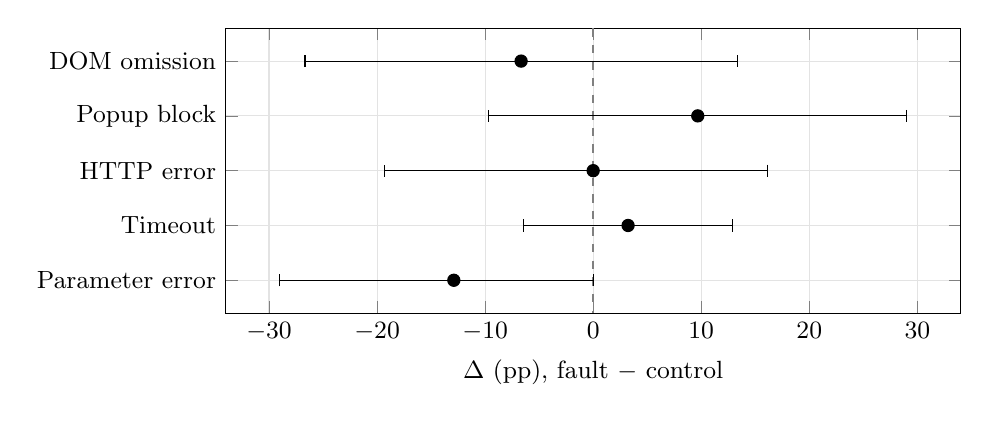
\begin{tikzpicture}
\begin{axis}[
  width=0.9\linewidth, height=5.2cm,
  xlabel={$\Delta$ (pp), fault $-$ control},
  ytick={1,2,3,4,5}, yticklabels={{DOM omission},{Popup block},{HTTP error},{Timeout},{Parameter error}},
  y dir=reverse, ymin=0.4, ymax=5.6,
  xmin=-34, xmax=34, xtick={-30,-20,-10,0,10,20,30},
  grid=major, grid style={gray!22},
  tick label style={font=\small}, label style={font=\small},
]
\draw[gray,dashed,thick] (axis cs:0,0.4) -- (axis cs:0,5.6);
\addplot[only marks, mark=*, mark size=2.2pt, black,
  error bars/.cd, x dir=both, x explicit]
  coordinates {(-6.67,1) -= (20.00,0) += (20.00,0) (9.68,2) -= (19.35,0) += (19.35,0) (0.00,3) -= (19.35,0) += (16.13,0) (3.23,4) -= (9.68,0) += (9.68,0) (-12.90,5) -= (16.13,0) += (12.90,0)};
\end{axis}
\end{tikzpicture}
\caption{Paired risk difference $\Delta$ in official success (fault $-$ control) on native-evaluator pairs, with the percentile bootstrap interval over pair units. Every interval spans zero and no fault survives Holm correction, which is the paper's primary result. Compare Table~\ref{tab:official_native}.}
\label{fig:forest}
\end{figure}
